%Préambule du document :
\documentclass[12pt, a4paper]{book}
%\usepackage[latin1]{inputenc} 

\usepackage[T1]{fontenc} % | "`pipe"' character
\usepackage{graphicx}
\usepackage{titling}
\usepackage{amssymb} 
\usepackage{minitoc} % chapter's tocs
\usepackage{authblk} % author affiliations
\usepackage{fancyhdr} % modify the headers
\usepackage{tabularx} % tables not larger than A4
\usepackage[table]{xcolor} %colours inside the tables
\usepackage{float}
\usepackage{multicol} % multiple columns in some sections
\usepackage[inner=2cm,outer=2cm]{geometry} %A4 margins

\usepackage[labelfont=bf, margin=0.5cm]{caption} % for figure captions in minipages
\usepackage{hyperref} %link references (toc, citations) inside document
\usepackage{natbib} % to cite with parentheses and plain text et only year if you please...
\usepackage{amsmath}
 \usepackage{fixltx2e} % allows overrightarrow to be in caption
 \MakeRobust{\overrightarrow}




\bibliographystyle{plainnat} % reference style
\renewcommand{\bibname}{References} %Rename "`bibliography"' => "`references"'

\hypersetup{
    colorlinks,
    citecolor=brown,
    filecolor=green,
    linkcolor=red,
    urlcolor=blue
}
\hypersetup{linktocpage}


\pagestyle{fancy}
\fancyhead{}
\fancyfoot{}
\fancyhead[RO,LE]{\thepage}
\fancyhead[LO]{\leftmark}
\fancyhead[RE]{\rightmark}
\setcounter{tocdepth}{1} % we only want chapters and sections in toc
\setcounter{minitocdepth}{1} %we only want sections in chapters' minitocs

\pretitle{%
  \begin{center}
  \LARGE
  
\includegraphics[width=12cm]{Logo_software.png}\\[\bigskipamount]
}
\posttitle{\end{center}}

\title{ISE-MeshTools User's guide\\ISE-MeshTools v1.3}



%\titlepicture[width=13cm]{Logo_software.png}
\author{Renaud LEBRUN}
\affil{Institut des Sciences de l'Evolution, University of Montpellier, France}
\date{\today} 


%Corps du document :
\begin{document}

	\dominitoc

\maketitle
 

\tableofcontents

\chapter*{Introduction}
\addstarredchapter{Introduction}

\markboth{INTRODUCTION}{}

\minitoc 

 ISE-MeshTools \citep{Lebrun2014} was developed  as a help to the scientific journal MorphoMuseuM (M3), in order to help scientists to produce enriched surface The source code is hosted on Github. 
\section*{Origin of the project}
\addcontentsline{toc}{section}{Origin of the project}
Over the last two decades, even though 3D data acquisition and computer-assisted techniques have grown increasingly popular among biologists, paleontologists and paleoanthropologists, so far, no standard biology-oriented 3D mesh manipulation software has emerged; most of the time, researchers either use commercial software which are not primarily designed for biologists, or develop their own in-house software solutions. ISEM-MeshTools is developed to meet the need to ease the production and the diffusion of 3D models of biological organisms. ISE-MeshTools provides a set of tools for editing, positioning, deforming, labelling, tagging sets of 3D surfaces. As such, ISE-MeshTools can be used to produce enriched models which can in turn be submitted to M3.
\section*{Main features}
\addcontentsline{toc}{section}{Main features}
Features include:
\begin{itemize}
\item Retro-deformation for virtual restoration of fossils/deformed specimens;
\item Point and curve primitives for placing the exact type of landmark points you’re interested in
\item Easy to use 3D interface for positioning and manipulating sets of surfaces and landmark primitives
\item Mesh tagging, labelling and colouring (to allow for the creation of anatomy atlases)
\item Mesh scalar computation and colouring (based upon curvature/thickness etc...)
\end{itemize}

 ISE-MeshTools allows to import and export 3D meshes in standard formats such as STL, PLY and VTK, and as such, in can be used in conjunction with a variety of other 3D mesh editors such  as MeshLab (http://meshlab.sourceforge.net/) or Blender (https://www.blender.org/) 
\section*{Implementation}
\addcontentsline{toc}{section}{Implementation}
ISE-MeshTools is entirely written in C++, and uses the visualization library VTK \citep{Avila2001}. The GUI has been designed with FLTK (FLTK, 1998). Since the end of 2015, ISE-MeshTools has become open-source and cross platform, and we are looking forward to welcoming new developers in the future in order to implement new functionalities. 


		 \chapter{Licence}
    
		\minitoc
		
    \section{ISE-MeshTools}
    ISE-MeshTools is Copyright(C) 2013-2016: Renaud LEBRUN, Cécile PELADAN, Stefan SCHLAGER, Jean DUMONCEL. All rights reserved.
This program is free software; you can redistribute it and/or modify it under the terms of the GNU 
General Public License as published by the Free Software Foundation; either version 2 of the License, 
or any later version.\\\\
This program is distributed in the hope that it will be useful, but WITHOUT ANY WARRANTY; without 
even the implied warranty of MERCHANTABILITY or FITNESS FOR A PARTICULAR PURPOSE. See the 
GNU General Public License for more details.

    \section{VTK}
  ISE-MeshTools’ compiled versions contain binary forms of VTK: Copyright (c) 2000-2006 Kitware Inc. 28 
Corporate Drive, Suite 204, Clifton Park, NY, 12065, USA. All rights reserved. Redistribution and use 
in source and binary forms, with or without modification, are permitted provided that the following 
conditions are met:\\
    Redistributions of source code must retain the above copyright notice, this list of conditions and 
the following disclaimer.\\
    Redistributions in binary form must reproduce the above copyright notice, this list of conditions 
and the following disclaimer in the documentation and/or other materials provided with the distribution.//
    Neither the name of Kitware nor the names of any contributors may be used to endorse or promote products derived from this software without specific prior written permission.\\\\
THIS SOFTWARE IS PROVIDED BY THE COPYRIGHT HOLDERS AND CONTRIBUTORS ``AS IS’’ AND ANY 
EXPRESS OR IMPLIED WARRANTIES, INCLUDING, BUT NOT LIMITED TO, THE IMPLIED WARRANTIES 
OF MERCHANTABILITY AND FITNESS FOR A PARTICULAR PURPOSE ARE DISCLAIMED. IN NO EVENT 
SHALL THE AUTHORS OR CONTRIBUTORS BE LIABLE FOR ANY DIRECT, INDIRECT, INCIDENTAL, SPECIAL, 
EXEMPLARY, OR CONSEQUENTIAL DAMAGES (INCLUDING, BUT NOT LIMITED TO, PROCUREMENT OF 
SUBSTITUTE GOODS OR SERVICES; LOSS OF USE, DATA, OR PROFITS; OR BUSINESS INTERRUPTION) 
HOWEVER CAUSED AND ON ANY THEORY OF LIABILITY, WHETHER IN CONTRACT, STRICT LIABILITY, 
OR TORT (INCLUDING NEGLIGENCE OR OTHERWISE) ARISING IN ANY WAY OUT OF THE USE OF THIS 
SOFTWARE, EVEN IF ADVISED OF THE POSSIBILITY OF SUCH DAMAGE.

		  \chapter{F.A.Q.}
  
    \section{How should I cite ISE-MeshTools in scientific publications ?}
    You may  cite ISE-MeshTools with the following reference :\\
		Lebrun, R. ISE-MeshTools, a 3D interactive fossil reconstruction freeware. 
		12th Annual Meeting of EAVP, Torino, Italy; 06/2014.
    \section{Is ISE-MeshTools a geometric morphometrics software ?}
    No. However, you can digitize 3D landmarks on complex 3D surfaces using ISE-MeshTools, which you 
		can use in other software.
		\section{Can I produce/extract 3D meshes out of CT/MRI data using ISE-MeshTools ?}
		No. To extract 3D meshes CT/MRI data sets, you have to use another software. However, you can edit 
		3D Meshes in various ways using ISE-MeshTools.
		\section{Is there a CTRL-Z functionnality around ?}
		No, there is currently no way to cancel any action. So remember to regularly save your work (especially when tagging surfaces), otherwise precious hours of work can be lost in a second.
     \chapter{Interaction modes}
\minitoc  

 \section{Selection modes}
 \subsection{Normal mode}
Press ``
\includegraphics{images/pixmap/Normal_select_mode.png}" to activate this mode.\\
This is the default selection mode. Selected objects (meshes and landmarks) are drawn ``grey". Unselected ``normal" landmarks are red, while ``target" landmarks are yellow. Unselected meshes can be drawn:
\begin{itemize}
\item Using a uniform colour (default modes)
\item According to tag values at each vertex (tag display mode active 
\includegraphics{images/pixmap/Show_Tag_Window.png})
\item	According to scalar values at each vertex (scalar display mode active 
\includegraphics{images/pixmap/show_color_scale.png} )
\end{itemize}



\subsection{Tag mode}
Press ``
\includegraphics{images/pixmap/Tag_select_mode.png}"to activate this mode
This mode is useful when tagging surfaces (as you can only interact with selected objects). Unselected meshes are drawn ``grey".  Unselected ``normal" landmarks are red, while ``target" landmarks are yellow. Selected landmarks are grey, while selected meshes can be drawn:
\begin{itemize}
\item	Using a uniform colour (default modes)
\item According to tag values at each vertex (tag display mode active 
\includegraphics{images/pixmap/Show_Tag_Window.png})
\item	According to scalar values at each vertex (scalar display mode active 
\includegraphics{images/pixmap/show_color_scale.png} )
\section{Interaction modes}
\end{itemize}

\subsection{Camera mode}
  
\includegraphics{images/pixmap/move.png}``Camera mode" is the default interaction mode, and is active on startup. When active, left and middle mouse button drags result in camera rotation/translation, respectively.
\subsection{Object mode}
   
\includegraphics{images/pixmap/move_mode2.png}When active, left and middle mouse button drags result in object rotation/translation, respectively.
\subsection{Landmark mode}
  
\includegraphics{images/pixmap/Landmarks2.png}When active, only landmarks can be selected/unselected via right mouse button drag/click. This mode is useful when editing/placing landmarks. Left and middle mouse button drags result in camera rotation/translation, respectively.

\section{Landmark setting modes}
Landmarks can be set on surfaces by pressing ``L" + left mouse click. 
Two series of conventional landmarks can be set with ISE-MeshTools: ``normal" and ``target" landmarks. Additionally a third landmark series (``flag" landmarks) can be used to label surface structures. 
\subsection{Normal landmark mode}	
Press ``
\includegraphics{images/pixmap/Landmarks4.png}" to activate this mode (this mode is active by default)
\subsection{Target landmark mode}	

Press ``
\includegraphics{images/pixmap/Landmarks6.png}"  to activate this mode
\subsection{Flag landmark mode}	

Press ``
\includegraphics{images/pixmap/Flag01.png}" to activate this mode

	   \chapter{Keyboard and mouse controls}
\minitoc  

 \section{Keyboard and mouse controls}
\rowcolors{2}{}{gray!25}
\begin{tabularx}{\linewidth}{ | c | X | }
 \hline			
   Ctrl+A & Selects all objects \\ \hline				
   Ctrl+D & Unselects all objects \\ \hline				
   L+ left click & Creates a landmark (either ``normal", ``target" or ``flag" landmark). \\ \hline			
L + right click & If a single landmark is selected, its position is
moved. Nothing happens if no landmark is selected
or if more than one landmark are selected \\ \hline			

Left mouse button drag 
& Camera mode : camera rotation.\newline
 Object mode : object rotation.\newline
Landmark mode : camera rotation. \\ \hline			

Ctrl + left mouse button drag 
& Camera mode : object rotation.\newline
 Object mode : camera rotation.\newline
 Landmark mode : object rotation. \\ \hline	
		
Right mouse button drag & Draws a yellow rectangle. Once right button is
released, all objects (surfaces and landmarks)
falling inside the rectangle get selected/unselected,
depending on their initial selection status \\ \hline	
		
Right mouse button click & All objects (surfaces and landmarks) lying at click
location get selected/unselected, depending on
their initial selection status \\ \hline		
	
Middle mouse button roll (roll wheel) & Zoom / unzoom \\ \hline		
	
Middle mouse button drag 
& Camera mode : camera translation\newline
 Object mode : object translation\newline
 Landmark mode : camera translation \\ \hline	
		
Ctrl + middle mouse button drag 
& Camera mode : object translation\newline
Object mode : camera translation\newline
Landmark mode : object translation \\ \hline			

« Del » & All selected objects are deleted \\ \hline			

T + left click & Tag selected surface with active tag value \\ \hline			
 
T + right click & Tag selected surface with ``0" value \\ \hline			

 \end{tabularx}

\section{Additional controls}
Additional controls are available when using ``lasso cut" or ``lasso tag" (lasso mode should be active):\\
\begin{tabularx}{\linewidth}{ | c | X | }
\hline			
Left click & Adds a segment to polygon (segments are drawn yellow) \\ \hline			

Right click & Connects last segment to first segment. If two segments cross each other, lasso action is canceled. Otherwise, the closed polygon is drawn red.\\ \hline			

Middle click or ``C" + right click. & Once the lasso is closed (lasso polygon drawn red
after a right click), all the vertices falling within the clicked region (outside or inside the polygon) are either:\newline
- given the colour corresponding the the active tag (lasso tag)\newline
- inserted into a new objects (lasso cut).\newline 
See lasso cut and lasso tag sections for further information.\\ \hline	
		
T + left click (``lasso tag" only) & Depending on which tag tool is active, if the
lasso is closed (lasso polygon drawn red after a right click) the vertices are painted either :\newline 
- using the pencil\newline 
- using the magic wand\newline 
- using the flood fill\newline 
Tag propagation is restricted within the area defined by the red polygon.\\ \hline		
	
\end{tabularx}


		 \chapter{Camera and object GUI main controls}
\minitoc  

 \section{Camera controls}
\subsection{Camera rotation centre}
By default, the camera rotates around the origin of the coordinate system (x=0, y=0, z=0), but by pressing ``
\includegraphics[scale=0.7]{images/pixmap/Move_cam.png}", the camera will revolve around the centre of mass of all opened objects. The latter option is useful when the centre of mass of an object (or of several ones) is far from the origin of the coordinate system. The grid is drawn using different colors depending on the camera rotation centre (see Fig. \ref{grid_color}). The camera centre can also be set at the location of one of the first 10 ``normal" landmarks (see section \ref{camera_centre_at}).

\begin{figure}
  \centering
  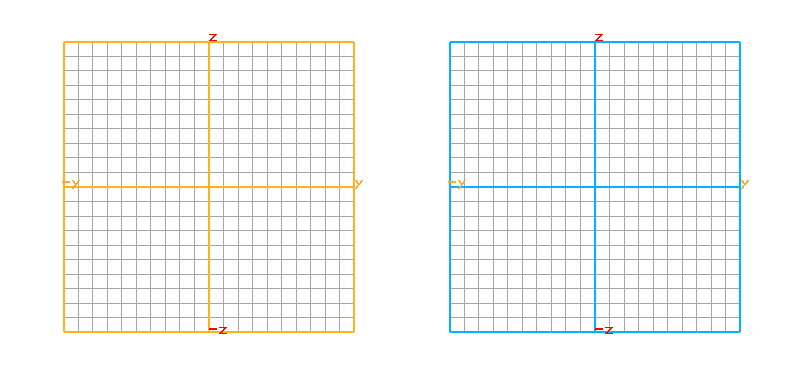
\includegraphics[scale=0.4]{images/GUI/Camera_rotation_centre.png} 
	\caption{Grid display coulour. Left: when the camera revolves around the origin of the coordinate system (x=0, y=0, z=0), the grid is displayed in orange. Right: when the camera revolves around the centre of mass of all opened objects, the grid has a blue layout.}
\label{grid_color}
 
\end{figure}

\subsection{Zoom}
There are three ways to modify the ``zoom" in ISE-MeshTools :


\begin{minipage}{0.7\textwidth}
\begin{itemize}
\item You may use the zoom roller laying in the lower part of the right panel of the main window.
\item	You may open the camera options window (viewing opt. $\rightarrow$  Camera $\rightarrow$ Camera options) and modify manually the ``Zoom" control.
\item	You may set manually the display scale (viewing opt $\rightarrow$ Camera $\rightarrow$ Set 100 pixels in mm)
\item	You may use the middle click mouse roll button (roll the wheel).
\end{itemize}
\end{minipage}    
\begin{minipage}{0.25\textwidth}\centering
  
\includegraphics[scale=0.5]{images/Icons/zoom_01.png}
 \captionof{figure}{Zoom Roll}
 \end{minipage}    


When the option ``Adapt field of view depth" is active in the Rendering options window (Viewing opt.$\rightarrow$General rendering options $\rightarrow$ Depth of field of view panel), changing the zoom value will also modify the depth of the field of view (camera.far value) and the position of the clipping plane (camera.tz value). When the option ``Keep current field of view depth" is active, changing the zoom will not affect the camera.far and camera.tz values.

\subsection{Camera rotation around ``z" viewing axis}

\begin{minipage}{0.7\textwidth}
To do so, you may use the slider lying in the upper part of the right panel of the main window.
\end{minipage}    
\begin{minipage}{0.25\textwidth}\centering
  
\includegraphics[scale=0.5]{images/Icons/Rotation_z.png}
 \captionof{figure}{Camera ``z" rotation slider}
 \end{minipage}    



\subsection{Clipping plane}

\begin{minipage}{0.7\textwidth}
In some cases, you may need to displace the viewing clipping plane. To do so, use
the slider lying centrally in the right panel of the main window.\\
You can also modify the clipping plane manually by editing the ``Tz" control in
the camera options window (viewing opt. $\rightarrow$ Camera $\rightarrow$ Camera options).
The buttons 
\includegraphics[scale=0.7]{images/Icons/clipping_plane3.png} and 
\includegraphics[scale=0.7]{images/Icons/clipping_plane2.png} which lie just underneath the clipping plane slider (and
also in the camera option window) also permit to adjust / readjust the position of
the clipping plane at predefined positions :
\begin{itemize}
\item  
\includegraphics[scale=0.7]{images/Icons/clipping_plane3.png}: the clipping plane is placed at z = 0 (all objects having a z coordinate along
z viewing axis smaller than 0 are hidden).
\item	
\includegraphics[scale=0.7]{images/Icons/clipping_plane2.png} : the clipping plane is replaced at its original value : z= - camera.far / 2. This value permits to
view objects having positive and negative coordinates along z viewing axis.

\end{itemize}
\end{minipage}    
\begin{minipage}{0.25\textwidth}\centering
  
\includegraphics[scale=0.5]{images/Icons/clipping_plane.png}
 \captionof{figure}{Camera clipping plane slider}
 \end{minipage}   




\subsection{Camera orientation}
6 camera positions are predefined :\\

\includegraphics[scale=0.7]{images/pixmap/right2.png} view object from right side \\

\includegraphics[scale=0.7]{images/pixmap/left2.png} view object from left side\\

\includegraphics[scale=0.7]{images/pixmap/right2.png} view object from front side (default camera position)\\

\includegraphics[scale=0.7]{images/pixmap/front2.png} view object from back side\\

\includegraphics[scale=0.7]{images/pixmap/above2.png} view object from above\\

\includegraphics[scale=0.7]{images/pixmap/back2.png} view object from below\\

\subsection{Coordinate system orientation helper}
\begin{minipage}{0.7\textwidth}
Press 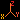
\includegraphics[scale=0.7]{images/pixmap/grid2.png} to show / hide the coordinate system orientation helper lying on the bottom left corner of the main 3D window. By default, the labels are defined
the following way:\\
+z axis : dorsal side\\
-z axis : ventral side\\
+y axis : left side\\
-y axis : right side\\
+x axis : proximal side\\
-x axis : distal side.\\
You may edit these labels depending on your preferences (for instance,
depending on the structure you are working with, you may need to set ``+y" to ``labial", and ``-y" to
``lateral"). To edit orientation labels, click on ``viewing opt. $\rightarrow$ Orientation labels."
\end{minipage}    
\begin{minipage}{0.3\textwidth}\centering
 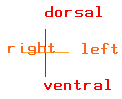
\includegraphics[scale=0.7]{images/GUI/Helper.png}
 \captionof{figure}{Orientation helper}
 \end{minipage}   

\subsection{Grid}
Press 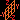
\includegraphics[scale=0.7]{images/pixmap/grid3.png} to show / hide the grid. Default grid size is 1 cm / square. Grid size can be edited manually
(viewing opt. $\rightarrow$ Grid size).
Switching between the 6 camera predefined positions defined above (
\includegraphics[scale=0.7]{images/pixmap/right2.png},
\includegraphics[scale=0.7]{images/pixmap/left2.png},
\includegraphics[scale=0.7]{images/pixmap/right2.png}, 
\includegraphics[scale=0.7]{images/pixmap/front2.png}, 
\includegraphics[scale=0.7]{images/pixmap/above2.png} and 
\includegraphics[scale=0.7]{images/pixmap/back2.png})will
affect the plane in which the grid is drawn.

\subsection{Lightning}
6 lightning orientations are predefined :\\

\includegraphics[scale=0.7]{images/pixmap/s_right_17.png}light from right viewing side\\

\includegraphics[scale=0.7]{images/pixmap/s_left_17.png}light from left viewing side\\

\includegraphics[scale=0.7]{images/pixmap/s_face_17.png}light from front viewing side\\

\includegraphics[scale=0.7]{images/pixmap/s_back_18.png}light from back viewing side\\

\includegraphics[scale=0.7]{images/pixmap/s_dessus_18.png}light from above\\

\includegraphics[scale=0.7]{images/pixmap/s_dessous_18.png}light from below\\

  \section{Object controls controls}
	As seen earlier, selected objects can be translated and rotated using the mouse left and middle buttons
(in landmark and camera selection modes, you also need to maintain ``CTRL" button pressed
while dragging the mouse to achieve rotation and translation of selected objects). Alternatively, you
may also use the following controls to accomplish rotation and translation of selected objects. Rotation
is performed around the global center of mass of all selected objects.

\subsection{Rotation around and translation along ``z" viewing axis}

\begin{minipage}{0.7\textwidth}
These controls are extremely useful, as there is no way to achieve rotation
around « z » viewing axis or translation along ``z" viewing axis using the
mouse. \\
To do so, use the slider and roller lying in the upper part of the left panel of the
main window.

\end{minipage}    
\begin{minipage}{0.25\textwidth}\centering
  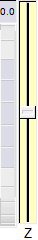
\includegraphics[scale=0.5]{images/Icons/x_rot.png}
 \captionof{figure}{Object ``z" rotation roller and slider}
 \end{minipage}    


\subsection{Rotation around ``x" and translation along ``y" viewing axes}

\begin{minipage}{0.7\textwidth}
To do so, use the slider and roller lying in the lower part of the left panel of the
main window.
\end{minipage}    
\begin{minipage}{0.25\textwidth}\centering
  \includegraphics[scale=0.5]{images/Icons/y_rot.png}
 \captionof{figure}{Object ``x" roller and ``y" slider}
 \end{minipage}   

\subsection{Rotation around ``y" and translation along ``x" viewing axes}


\begin{minipage}{0.5\textwidth}
To do so, use the slider and roller lying in the left part of the bottom panel of the
main window.
\end{minipage}    
\begin{minipage}{0.4\textwidth}\centering
  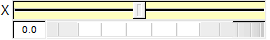
\includegraphics[scale=0.5]{images/Icons/z_rot.png}
 \captionof{figure}{Object ``y" roller and ``z" slider}
 \end{minipage}   


		 \chapter{Menu File}
\minitoc  

\section{Open surface}
.stl, .ply, .vtk surfaces can be open via this menu. ISE-MeshTools does not manage textures associated with meshes; still, you can open .obj files, but associated textures will not be loaded. When opening a .ply file containing RGB colours (for instance a file painted manually or automatically with ``MeshLab") or a .vtk file containing RGB scalars, these colours are placed inside the ``RGB" scalars. MeshTools will reinitialize the ``RGB" scalars whenever you change the object's colour or whenever you activate tag display mode or scalar display mode : if these colours are important to you, you may convert them to TAG values in the menu Tags$\rightarrow$Convert RGB colours to tags before changing the object colour or display mode/before changing tags or any colour scale activated.

\section{Save surface}
Selected surfaces can be saved into files. If no surface is selected, the following message appears:\\
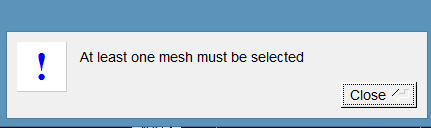
\includegraphics[scale=0.5]{images/File/Save_message.png}
If more than one mesh are selected, the following message shows up:\\
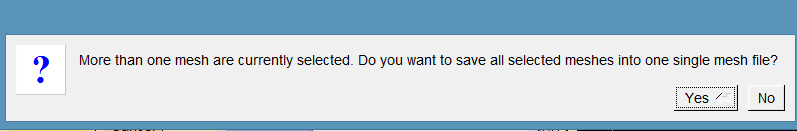
\includegraphics[scale=0.5]{images/File/Save_message2.png}

\subsection{Save .ply}

\begin{minipage}{0.5\textwidth}
Options:
\begin{itemize}
\item File type: you can save .ply data in binary (little or big endian)
or ASCII formats.
\item Position : you can keep object original coordinate system or
save the surface in its current position.
\item Normales : you can chose whether you wish to save normales.
\end{itemize}

\end{minipage}    
\begin{minipage}{0.5\textwidth}\centering
  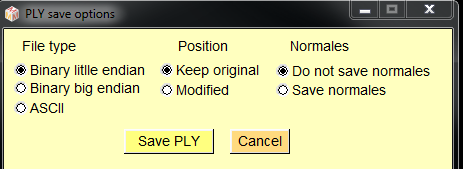
\includegraphics[scale=0.45]{images/File/Save_ply_new.png}
 \captionof{figure}{PLY save options window}
 \end{minipage} 

Note that the ``RGB" scalar (object rendering colour, depending on which rendering mode you
are using) will be saved inside the .ply file. This means that Tag / Scalar / Object colour can be exported and viewed in other software such as MeshLab.


\subsection{Save .stl}

\begin{minipage}{0.5\textwidth}
Options:
\begin{itemize}
\item File type: you can save .stl data in binary (little endian) or
ASCII formats.

\item Position : you can keep object original coordinate system or save the surface in its current position
\end{itemize}

\end{minipage}    
\begin{minipage}{0.5\textwidth}\centering
  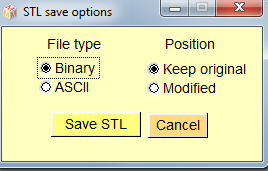
\includegraphics[scale=0.5]{images/File/Save_stl.png}
 \captionof{figure}{STL save options window}
 \end{minipage} 





\subsection{Save .vtk}
\begin{minipage}{0.5\textwidth}
Vtk mesh file format is by far not as widespread as stl or ply
format. However, it is extremely useful as it allows to store
scalar and tag values at each vertex or at each triangle.
Options:
\begin{itemize}
\item File type: you can save .vtk data in binary (little endian) or
ASCII formats.

\item Position : you can keep object original coordinate system
or save the surface in its current position
\end{itemize}
\end{minipage}    
\begin{minipage}{0.5\textwidth}\centering
  \includegraphics[scale=0.5]{images/File/Save_vtk.png}
 \captionof{figure}{VTK save options window}
 \end{minipage} 
\noindent
Note that the ``RGB" scalar (object rendering colour, depending on which rendering mode you are
using) will be saved inside the .vtk file.
\subsection{Save .obj}

\begin{minipage}{0.5\textwidth}
ISE-MeshTools does not manage textures associated with
meshes. Still, you can save meshes in .obj format, but
textures will not be saved.
Options:
\begin{itemize}
\item Position : you can keep object original coordinate system
or save the surface in its current position
\end{itemize}
\end{minipage}    
\begin{minipage}{0.5\textwidth}\centering
  \includegraphics[scale=0.5]{images/File/Save_obj.png}
 \captionof{figure}{OBJ save options window}
 \end{minipage} 


\section{Position}
In ISE-MeshTools, mesh position consists in two
4*4 square matrices: one matrix is used as the
aspect matrix (by default the identity matrix),
and the other one as the position matrix. These
matrices can be opened and saved in ``.pos"
format (see Fig. \ref{position_file}).


\begin{figure}
  \centering
  \includegraphics[scale=0.5]{images/File/Position_file.png}
 \caption{Example of .pos position file. The first 4 lines correspond
to the aspect matrix, and the 4 last lines to the position matrix.}
\label{position_file}
\end{figure}
 



\subsection{Load position}
If no surface is selected, the following message
appears:\\
\includegraphics[scale=0.5]{images/File/open_position1.png}
\\
If more than one mesh are selected, the following message shows up :\\
\includegraphics[scale=0.5]{images/File/open_position2.png}

\subsection{Load transposed position}
This option may be useful in the following case:
\begin{itemize}
\item Let us suppose that you did modify the position of a given surface and saved its position
\item Then you have saved the surface in its current modified position (that is : the original position of the
surface is lost).
\end{itemize}

For some reason, you may need to open the surface in its original position. To do so, you may apply this option (apply transposed position matrix to the modified surface).
Note : this option only works if the aspect matrix was not modified.

\subsection{Save position}
Mesh aspect and position matrices can be saved in ``.pos" format. If no surface is selected, the
following message appears:\\
\includegraphics[scale=0.5]{images/File/save_pos1.png}
\\
If more than one mesh are selected, the following message shows up:\\
\includegraphics[scale=0.5]{images/File/save_pos2png.png}

\subsection{Edit manually aspect and position matrices}
There are two ways to access the object matrix editor :
\begin{itemize}

\item Either select one surface and click on ``\includegraphics[scale=0.7]{images/pixmap/mat.png}"(edit first selected object position and aspect matrices).
\item Or select one surface and click on ``edit selected surfaces$\rightarrow$Rendering modifications$\rightarrow$ edit first
selected object position and aspect matrices".
\end{itemize}



This opens the ``Object Matrix" window, in which the aspect and position matrices can be edited. See ``Edit selected surfaces" section \ref{edit_mat_section} (Rendering modifications$\rightarrow$ edit first selected object position and aspect matrices) for further information.


\section{Project}




When working with multiple surface objects,
loading surfaces and associated positions one
by one becomes fastidious. You may open and
save series of meshes and associated position
matrices using this menu.
``project" files (.ntw) files are organized the
following way (see Fig. \ref{project_file}):
- Name of surface 1 file\\
- Name of position 1 file associated to surface 1\\
- Surface 1 RGB colour and transparency\\
- Name of surface 2 file\\
- Name of position 2 file associated to surface 2\\
- Surface 2 RGB colour and transparency (etc...)\\
 


Surface files can be of the following types : .stl, .vtk, .ply and .obj\\
``.ntw" files can be constructed manually, providing that the refered surface and position files exist.



\begin{figure}
  \centering  
 \includegraphics[scale=0.7]{images/File/Ntw.png}
 \captionof{figure}{Example of project .ntw file}
\label{project_file}
\end{figure}

\subsection{Open project}
Loads a .ntw file

\subsection{Save project}
Saves a .ntw file implicating all selected surfaces. Though ISE-MeshTools can open .ntw files
implicating .stl, .ply and .obj surfaces, when saving a .ntw project, surface files will be saved in .vtk format in order to keep potential tag / scalars associated to each saved surface. Each surface file will be given the name of the original file. Each position file will be given a name which starts with the name of the associated surface and ends with the name of the project. In the .ntw file example shown above, the surface files are 
\begin{itemize}
\item ``Seg-SP07-URM2\_EDJ2.vtk" 
\item ``Seg-SP07-URM2\_OES2.vtk"
\end{itemize}
\noindent and the project name is ``M2\_Sup.ntw". The advantage of naming position files that way is you may construct different .ntw files with different associated surface files using a same set of surfaces.\\
\noindent
\begin{minipage}{0.6\textwidth}
\noindent \noindent Requirement : all selected surfaces saved via this option
need to have distinct names.
Note : When working with ``project" files, you may need at
some point to rename some of the object surfaces. To do so,
select one surface, click on \includegraphics[scale=0.7]{images/pixmap/name.png}: the ``Edit Name" window appears.
Press ok to modify the name of that surface object.
See tutorial ``working with projects" for further information.
\end{minipage}  
 \begin{minipage}{0.4\textwidth}\centering
  \includegraphics[scale=0.5]{images/Icons/edit_name.png}
 \captionof{figure}{Edit name window}
 \end{minipage} 


\section{Landmarks}
As mentioned earlier, landmarks can be set on surfaces by pressing ``L" + left mouse click.\\

Two series ofconventional landmarks can be set : ``normal" and ``target" landmarks. As mentioned earlier, in the ``normal" landmark mode (button \includegraphics[scale=0.7]{images/pixmap/Landmarks4.png} active), pressing ``L" + left mouse click results in
the creation a ``normal" landmark (a red one). In the ``target" landmark mode (button \includegraphics[scale=0.7]{images/pixmap/Landmarks6.png} active),
pressing ``L" + left mouse click will create a ``target" landmark (a yellow one). ``Normal" and ``target" landmarks can be loaded and saved.\\
Selected ``normal"/"target" landmarks can be reordered using the following buttons. Pressing ``\includegraphics[scale=0.7]{images/pixmap/s_dessous_17.png}"
will place the selected landmarks earlier in the ``normal"/"target" landmark list, while pressing ````\includegraphics[scale=0.7]{images/pixmap/s_dessus_17.png}""
will place them one step further, respectively.\\
ISE-MeshTools can manage two types of landmark files: ``.LMK" ``.VER" files.\\ .LMK files contain a series of lines, each line
being constructed the following way (see Fig. \ref{LMK_file}): landmark
name (without space or tab character),
landmark coordinates. Note that each landmark name does not need to be of the form ``landmark"+landmark number. Meanwhile, the name should not hold space or tab
characters.
\\
.VER files contain a series
of lines, each line being
constructed the following
way (see Fig. \ref{VER_file}): landmark name (without space or tab character), landmark coordinates, landmark orientation.

\begin{figure}
  \centering
  \includegraphics[scale=0.7]{images/Landmarks/LMK_file.png}
 \caption{Example of .LMK file}
\label{LMK_file}
\end{figure}

\begin{figure}
  \centering
  \includegraphics[scale=0.7]{images/Landmarks/VER_file.png}
 \caption{Example of .VER file}
\label{VER_file}
\end{figure}


\subsection{Load landmarks}
Landmarks opened using this option will be put in the ``normal" landmark list (red landmarks)
\subsection{Save landmarks}
You may decide whether you wish to save only selected ``normal" landmarks or all selected and
unselected ``normal" landmarks (the red ones).
\subsection{Save target landmarks}

You may decide whether you wish to save only selected ``target" landmarks or all selected and
unselected ``target" landmarks (the red ones).
The ``Landmarks" chapter (chapter \ref{landmark_chapter}) and the tutorial ``working with landmarks" contain further information regarding landmark digitization with ISE-MeshTools

\section{Curves}\label{file_curve_section}
3D Curves are constructed in ISE-MeshTools using 2 series of landmarks : a series of ``normal"
landmarks, and a series of ``target" landmarks of equal sizes. ``Target" landmarks are referred to as
``curve handles", when they are used to construct curves (``Target" landmarks can also be used to
achieve TPS deformation, see later in this documentation). By default, curves are not drawn in the
main 3D window : curves start being drawn when the checkbox ``draw curves" is checked in the menu
``Viewing opt." (\includegraphics[scale=0.7]{images/Landmarks/Draw_curves.png}). Curves are draw green when no landmark/curve handle belonging to
the curve is selected. Curves are drawn red when at least one landmark / curve handle involved in the
curve is selected. Two different cases are considered:
\begin{itemize}

\item Case 1: the numbers of ``normal" and ``handle/target" landmarks differ. In that case, a curve is a series of lines passing through ``normal" landmarks.
\item Case 2: the numbers of ``normal" and ``handle/target" landmarks differ. In that case, a curve is a
series of cubic Bezier curves passing through ``normal" landmarks. For a given set of 2 ``normal"
consecutive landmarks (Ln and Ln+1) and their associated curve ``handles" (Hn and Hn+1), a mirror
image of Hn+1 relative to Ln+1 (H'n+1) is constructed. The Bezier curve involving Ln, Ln+1, Hn and
Hn+1 starts from Ln, going toward Hn, and arrives at Ln+1 coming from the direction of H'n+1.

\end{itemize}


The explicit form of the curve is :
\begin{equation}
B(t) = (1-t)^{3}Ln + 3(1-t)^{3}tHn + 3(1-t)t^{2}H'n+1 +t^{3}Ln+1, t \in[0,1]
\end{equation}
In order to be able to digitize several curves using a given set of normal and target landmarks,
``normal" landmarks curves can be given 4 flags (see section \ref{landmarks_curves_section} ``Landmarks $\rightarrow$ Landmarks
involved into curves" for further details):\\
Flag ``0" : landmark is placed inside the curve (drawn ``red").\\
Flag ``1" : landmark is a curve start (drawn ``green").\\
Flag ``2" : landmark is placed inside the curve, and is a curve ``milestone" (drawn blue) .\\
Flag ``3" : landmark is placed inside the curve, and should be connected to the preceding curve
starting point. When landmark n is flagged that way, landmarkn+1 will be set as a curve starting point.\\
Flag ``2" is used to decompose a given curve into curve segments (see ``export curves as landmark file"). By default, a curve comprises 1 segment\\
Flag ``3" is used to close a curve (by default, curves are open).\\
3D curves are loaded and saved into .CUR files, which contain a series of lines, each line being
constructed the following way: name (without space or tab character), curve ``normal" landmark
coordinates, curve ``handle" coordinates, flag.
In the example shown below, 4 curves are defined :\\
- an open curve starting from landmark 1 and ending at landmark 7\\
- a closed curve involving landmarks 8 to 12\\
- a closed curve involving landmarks 13 to 20\\
- a closed curve involving landmarks 21 to 26\\
These four curves contain only one segment (no curve milestone was set within those 4 curves).
Note that each name does not need to be of the form ``landmark"+ number. Meanwhile, the name
should not hold space or tab characters.
\begin{figure}[t] 
  \centering
  \includegraphics[scale=0.5]{images/Landmarks/CUR_file.png} 
	\caption{Example of .CUR file}
 
\end{figure}

\subsection{Load curves}
This menu allows the user to load a .CUR file.
\subsection{Save curves}
This menu allows the user to save current landmarks and curve handles as a .CUR file. This action is only allowed if the number of ``normal" landmarks and ``target" landmarks is the same. If not, the following message appears:\\
\includegraphics[scale=0.5]{images/Landmarks/Not_identical.png}

\subsection{Export curves as landmark file}
\begin{minipage}{0.55\textwidth}

Curves can be transformed in a series of equidistant
landmarks using this option. The curve decimation window
appears.
Each curve/curve segment is saved as a number of
equidistant landmarks. In the present example, each curve/
curve segment is saved as 20 equidistant landmarks.

\end{minipage}  
 \begin{minipage}{0.45\textwidth}\centering
  \includegraphics[scale=0.5]{images/Landmarks/Export_curves.png}
 \captionof{figure}{Curve decimation window}
 \end{minipage} 

When pressing ``Ok", if the numbers of ``normal" landmarks and ``target" landmarks differ, the
following message appears:\\
\includegraphics[scale=0.5]{images/Landmarks/Can_not_export.png}

\subsection{Save curve infos (length per curve ...)}
\begin{minipage}{0.55\textwidth}

Each curve /curve segment length can be saved as a .txt file
using this option.
The ``Landmarks" chapter (chapter \ref{landmark_chapter}) and the
tutorial ``Working with curves" contain further important
information regarding curve digitization with ISE-MeshTools.

\end{minipage}  
 \begin{minipage}{0.45\textwidth}\centering
  \includegraphics[scale=0.5]{images/Landmarks/Curve_infos.png}
 \captionof{figure}{Example of curve info file}
 \end{minipage} 



\section{Tags and flags}

\begin{minipage}{0.55\textwidth}
- Tag colours and names can be edited interactively by
clicking on \includegraphics[scale=0.7]{images/pixmap/Show_Tag_Window2.png}, which opens the tag window (see the chapter
``Tags" (chapter \ref{tags_chapter}) and the tutorial ``Working with tags" for
further information).\\
- By default, Tags are not visible. To activate/deactivate tag
display, click on \includegraphics[scale=0.7]{images/pixmap/Show_Tag_Window.png}\\
- Using ``Tag display mode" (\includegraphics[scale=0.7]{images/pixmap/Tag_select_mode.png}) is useful when editing
surface tags.\\
25 Tag names and associated colours can be defined in ISEMeshTools.
Tag colours files (.TAG) consist of 25 pairs lines,
each pair being constructed following way :\\
line 2*n: Tag name\\
line 2*n+1: Tag colour and transparency
\end{minipage}  
 \begin{minipage}{0.45\textwidth}\centering
  \includegraphics[scale=0.5]{images/Icons/Tags.png}
 \captionof{figure}{Example of .TAG file}
 \end{minipage} 

\noindent
\begin{minipage}{0.55\textwidth}
Regarding flags, as stated earlier, one series of ``flag landmarks" can be set in ISE-MeshTools (button \includegraphics[scale=0.7]{images/pixmap/Flag01.png} should
be pressed). To edit flag label, length and colour, select one
flag landmark, click on \includegraphics[scale=0.7]{images/pixmap/Flag02.png}. The ``edit flag" window appears.
Pressing ok will update the label, the colour and the
length associated to the selected flag, which in turn will be
unselected. If you wish to edit a second flag, select it and press ``Refresh". The current colour, length
and label of the newly selected flag will appear in the edit flag window.
\end{minipage}  
 \begin{minipage}{0.45\textwidth}\centering
  \includegraphics[scale=0.5]{images/Flags/Edit1flag.png}
 \captionof{figure}{Edit Flag window}
 \end{minipage} 
\noindent
Flags are saved using the .FLG file format, which consists of n pairs of lines constructed the following way :\\
line 2*n: Flag name\\
line 2*n+1: Flag coordinates, flag orientation, flag length and colour.

\subsection{Load tag colours and labels}
Select a .TAG file using this menu $\rightarrow$ Then open the tag window (\includegraphics[scale=0.7]{images/pixmap/Show_Tag_Window2.png}) : Tag labels, colours and
transparencies should have been updated.
\subsection{Save tag colours and labels}
This option saves the current state of tag labels, colours and transparencies in a .TAG file.

\subsection{Load flags}
Select a .FLG file using this menu

\subsection{Save flags}
This option saves the current flag landmarks into a .FLG file, regardless their selection status.

\section{Save infos (surface area, volume...)}
\noindent
\begin{minipage}{0.55\textwidth}

Surface area, volume, triangle number and
vertex number of selected surface objects can be
saved in a .txt file using this option.
\end{minipage}  
 \begin{minipage}{0.45\textwidth}\centering
  \includegraphics[scale=0.4]{images/File/Infos.png}
 \captionof{figure}{Example of info file}
 \end{minipage} 
\noindent

Note: surface objects should be closed in order to provide a correct estimation of object volume.
\section{Orientation labels}
The coordinate system orientation helper labels can be saved into ``.ORI" files, which are .txt files
containing 6 lines, 1 for each axis.


\subsection{Load orientation labels}
Select a .ORI file using this menu $\rightarrow$ Then open the orientation labels window window (Viewing opt;
Orientation labels) : the 6 orientation labels should have been updated.

\subsection{Save orientation labels}
This option saves the current state of orientation labels in a .ORI file.


		 




\chapter{Viewing Options}
\minitoc  

\section{General color and lightning options}

The general options window contains the following
sections:\\\\
\noindent
\begin{minipage}{0.55\textwidth}
\subsection{Windows}
These controls affect the default color of objects opened within ISE-MeshTools, the color of grid elements, and the background color.
\subsection{Light}
These controls affect the orientation of the light and specular, diffuse and ambient light parameters. By default surface back faces are not shown. Back face lighting can be enabled if the checkbox ``enable two sided lighting" is checked

\end{minipage}  
 \begin{minipage}{0.45\textwidth}\centering
  \includegraphics[scale=0.4]{images/Viewing_options/General_color.png}
 \captionof{figure}{Lightning and color options window}
 \end{minipage} 
\noindent






\section{General rendering options}
The rendering options window contains the following sections:\\\\


\noindent
\begin{minipage}{0.55\textwidth}
\subsection{Object rendering when moving object/camera}
\underline{Show full surface / scalars (slower):}  when active, surfaces are fully drawn when moving the object or the camera. This results in a better perception of object / camera
movements. This option is convenient when working with light surfaces.\\

\noindent
\underline{Show point cloud (faster)}: 3D surface rendering can be slow using the preceding option when working with:\\
- large number of surfaces simultaneously\\
- heavy surfaces (large number of triangle / vertices)\\

\end{minipage}  
 \begin{minipage}{0.45\textwidth}\centering
  \includegraphics[scale=0.4]{images/Viewing_options/Rendering_options.png}
 \captionof{figure}{Rendering options window}

 \end{minipage} 
\noindent
Also, rendering is slower when tag rendering mode is active (\includegraphics[scale=0.7]{images/pixmap/Show_Tag_Window.png}) or when scalar rendering mode is active (\includegraphics[scale=0.7]{images/pixmap/show_color_scale.png} ) . In order to increase rendering speed, surfaces can be rendered as a schematic point cloud when moving the object or the camera.


\subsection{Depth of field of view}
When the option ``Adapt field of view depth" is active, changing the zoom value will affect the depth of the field of view (camera.far value) and the position of the clipping plane (camera.tz value). When the option ``Keep current field of view depth" is active, changing the zoom will not affect the camera.far and camera.tz values.\\


\begin{figure}[t] 
  \centering
  \includegraphics[scale=0.25]{images/Examples/Clipping_plane.png} 
	\caption{Left : cranium and mandible of the type specimen of \textit{Pan paniscus}(downloadable at http://www.metafro.be/primates/panpaniscustype ) rendered with the clipping plane placed at its original position. Right : the same skull viewed using a clipping plane placed at the position of the sagittal plane, revealing inner structures such as the endocranium cavity. Note that the position of the specimen was modified so that the sagittal plane of the skull passes  through the point (0,0,0) and is perpendicular to the vector (0,1,0).}
 
\end{figure}


\noindent
\begin{minipage}{0.55\textwidth}
\section{Camera}
\subsection{Camera options}


- Camera near, Camera far : define near and far clipping -
planes of the camera\\
- Azimuth, Elevation, Twist : camera rotation parameters\\
- Tx, Ty, Tz : camera translation in x, y and z\\

The buttons \includegraphics[scale=0.7]{images/pixmap/Clipping_plane_z0.png} and \includegraphics[scale=0.7]{images/pixmap/Clipping_plane_normal.png} which lie underneath the Tz control(and also underneath the clipping plane slider in the main window) permit to adjust / readjust the position of the clipping plane at predefined positions :\\

\end{minipage}  
 \begin{minipage}{0.45\textwidth}\centering
  \includegraphics[scale=0.5]{images/Icons/camera_options.png}
 \captionof{figure}{Camera options window}

 \end{minipage} 
\noindent
- \includegraphics[scale=0.7]{images/pixmap/Clipping_plane_z0.png}: the clipping plane is placed at z = 0 (all objects having a z coordinate along z viewing axis smaller than 0 are hidden).\\
\noindent- \includegraphics[scale=0.7]{images/pixmap/Clipping_plane_normal.png}: the clipping plane is replaced at its original value : z= - camera.far / 2. This value permits to view objects having positive and negative coordinates along z viewing axis.

\subsection{Camera rotation centre at}\label{camera_centre_at}



Camera rotation centre can be set at the origin of the coordinate system (x=0, y=0, z=0) or at the location of one of the first 10 ``normal" landmarks.

\subsection{Set 100 pixels in mm}

\noindent
\begin{minipage}{0.55\textwidth}
Camera zoom can be modified in order to reach a desired display pixel size. This is useful to produce scaled images.

\end{minipage}  
 \begin{minipage}{0.45\textwidth}\centering
  \includegraphics[scale=0.5]{images/Icons/100px_mm.png}
 \captionof{figure}{Scale window\\}

 \end{minipage} 
\noindent


\subsection{Reset camera}
You may use this option to reinitialize camera parameters.
\section{Object rendering options}

\noindent
\begin{minipage}{0.55\textwidth}



\subsection{Gouraud shading}
This is the default rendering mode. Object rendering is performed using vertices' normals.

\end{minipage}  
 \begin{minipage}{0.45\textwidth}\centering




 \includegraphics[scale=0.1]{images/Viewing_options/Normal_gouraud.png}
 \captionof{figure}{Gouraud shading}

 \end{minipage} 
\noindent


\noindent
\begin{minipage}{0.55\textwidth}

\subsection{Draw wireframe}
This option can be useful to inspect the structure of the surface.

\end{minipage}  
 \begin{minipage}{0.45\textwidth}\centering

\includegraphics[scale=0.1]{images/Viewing_options/wireframe.png}
 \captionof{figure}{Example of wireframe rendering}

 \end{minipage} 
\noindent

\noindent
\begin{minipage}{0.55\textwidth}
\subsection{Sort vertices from back to front}\label{sort_back_front}
This option is (only) useful when working with transparent surfaces, in the case you want to display all surface inner structures. When active, whenever the camera of the
object is moved, vertices will be sorted in order to be displayed from back to front. This is the way transparency is achieved in OpenGL. As a consequence, rendering fluidity
becomes slow when working with heavy surfaces and/or a large number of objects. To change the transparency of an object, select an object, and reach ``Edit selected surfaces $\rightarrow$
Rendering modifications $\rightarrow$ Set alpha value".\\

Alternatively, in order to increase rendering fluidity, you may chose not to use the ``Sort vertices from back to front beware: slow rendering)" rendering option, but to sort episodically the vertices from back to front by pressing the button \includegraphics[scale=0.7]{images/pixmap/Sort_vertices01.png}.\\
Working with transparency is useful to observe inner structures and/or when digitizing landmarks
inside structures.

\end{minipage}  
 \begin{minipage}{0.45\textwidth}\centering

\includegraphics[scale=0.1]{images/Viewing_options/Sort_back_front.png}
 \captionof{figure}{Sort vertices from back to front.In this example, vertices are displayed from back to front. Four landmarks placed within this structure can be visualized.}

 \end{minipage} 
\noindent


\noindent
\begin{minipage}{0.55\textwidth}

\subsection{Sort vertices from front to back}\label{sort_front_back}
This option is (only) useful when working with transparent surfaces, and when you do not want to display too many inner structures. When active, whenever the camera of the object is moved, vertices will be sorted in order to be displayed from front to back. As a consequence, rendering fluidity becomes slow when working with heavy surfaces and/or a large number of objects. Alternatively, in order to increase rendering fluidity, you may chose not to use the ``Sort vertices from front to back (beware: slow rendering)" rendering option, but to sort
episodically the vertices from front to back by pressing the button \includegraphics[scale=0.7]{images/pixmap/Sort_vertices02.png}.

\end{minipage}  
 \begin{minipage}{0.45\textwidth}\centering

\includegraphics[scale=0.1]{images/Viewing_options/Sort_front_back.png}
 \captionof{figure}{Sort vertices from front to back.}

 \end{minipage} 
\noindent

\noindent
\begin{minipage}{0.55\textwidth}

\subsection{Flat triangles}
Using this option improves the perception of surface structure.

\end{minipage}  
 \begin{minipage}{0.45\textwidth}\centering
\includegraphics[scale=0.1]{images/Viewing_options/Triangles.png}
 \captionof{figure}{Example of flat triangle surface rendering}

 \end{minipage} 
\noindent

\noindent
\begin{minipage}{0.55\textwidth}

\subsection{Wireframe and flat triangles}
Using this option further improves the perception of surface structure.

\end{minipage}  
 \begin{minipage}{0.45\textwidth}\centering


\includegraphics[scale=0.1]{images/Viewing_options/Triangle_flat_triangles.png}
 \captionof{figure}{Example of flat triangle + wireframe surface rendering}

 \end{minipage} 
\noindent




\noindent
\begin{minipage}{0.55\textwidth}

\subsection{Backface culling}
Surface's back faces are hidden when using this option.
\end{minipage}  
 \begin{minipage}{0.45\textwidth}\centering

\includegraphics[scale=0.1]{images/Viewing_options/Backface_culling.png}
 \captionof{figure}{Backface culling rendering}

 \end{minipage} 
\noindent




\subsection{Display vertices ids}
For surface inspection purposes, you may sometimes need to visualize vertices ids. Note : this option affects rendering fluidity even when using relatively light surfaces.

\subsection{Display triangle ids}
For surface inspection purposes, you may sometimes need to visualize triangle ids.\\
Note : this option affects rendering fluidity even when using relatively light surfaces.\\



\noindent
\begin{minipage}{0.45\textwidth}\centering
\includegraphics[scale=0.1]{images/Viewing_options/Vertices_ids.png}
 \captionof{figure}{Gouraud shading + vertices ids rendering}

\end{minipage}  
 \begin{minipage}{0.45\textwidth}\centering
\includegraphics[scale=0.1]{images/Viewing_options/Triangle_ids.png}
 \captionof{figure}{Gouraud shading + triangle ids rendering}

 \end{minipage} 
\noindent





\section{Grid size}


\noindent
\begin{minipage}{0.55\textwidth}
Grid rendering can be edited to reach the desired size/square
\end{minipage}  
 \begin{minipage}{0.45\textwidth}\centering
\includegraphics[scale=0.5]{images/Viewing_options/Grid_size.png}
 \captionof{figure}{Grid size window}

 \end{minipage} 
\noindent





\section{Landmark and flag rendering options}
The landmark and flag options window (see Fig. \ref{landmarks_flags_options}) contains the following sections:

\subsection{Landmarks rendering}
``Normal" and ``Target" landmarks can be drawn as spheres or as needles. Landmark display size can be chosen to be adjusted automatically (default behaviour) or edited manually (when you feel that the automatic adjustment does not meet your needs) also edited manually in this section.



\subsection{Flags settings}
Flag length and color settings can be defined in thissubsection. Once placed on a surface and selected, the color, the length and the label of the flag can be changed by pressing
\includegraphics[scale=0.7]{images/pixmap/Flag02.png}.


\begin{figure}
  \centering  
 \includegraphics[scale=0.5]{images/Viewing_options/Landmark_options.png}
 \captionof{figure}{Landmark and flag options window.}
\label{landmarks_flags_options}
\end{figure}

\section{Display landmark numbers}
``Normal" and ``target" landmark numbers are displayed by default. For illustration purposes, you may sometimes need to hide landmark numbers.

\section{Draw curves}
Activate/deactivate this option to draw/hide 3D Bezier curves passing through ``normal" landmarks. See the tutorial ``working with curves" for further details regarding curve digitization with ISEMeshTools.

\section{Orientation labels}


\noindent
\begin{minipage}{0.55\textwidth}
The labels associated to the 6 orientation axes can be modified using this window. This will affect the coordinate system orientation helper displayed on the bottom left area of the 3D
window.

\end{minipage}  
 \begin{minipage}{0.45\textwidth}\centering
\includegraphics[scale=0.5]{images/Viewing_options/Object_labels.png}
 \captionof{figure}{Edit orientation labels window}

 \end{minipage} 
\noindent



\section{VBO activate (GPU acceleration)}
By default, ISE-MeshTools does not use the graphic card to display 3D objects, which slows down dramatically the rendering speed of heavy 3D meshes and that of tagged meshes. However, we have chosen not to activate the ``VBO" rendering option by default, as we have experienced that it causes ISE-MeshTools to crash on old computers or on some others which have not up to date graphic card drivers. By activating the graphic card acceleration option (VBO activate), you will probably find out that ISE-MeshTools is much more fluid to work with.\\ This feature was implemented by Cécile Peladan.


		 
\chapter{Edit selected surfaces}
\minitoc 


As a prerequisite, you need to select surfaces. Only selected surfaces can be edited. 



\section{Structure modifications}
\subsection{Invert}

A given surface's triangles can be
inverted in order to show inner structures (see Fig. \ref{inversion}).\\

Note that the original surface
is directly affected; this option
does not involve the use of a
filter (no output additional
surface is created).


\begin{figure}
  \centering
  \includegraphics[scale=0.4]{images/Edit_selected_objects/01_invert.png} 
	\caption{Example of surface triangle inversion. Left: original surface.
Right: the same surface inverted, revealing inner structures such
as the endocranial cavity. Gouraud shading rendering + backface
culling option was used.}
\label{inversion}
 
\end{figure}






\subsection{Mirror}

This option uses vtkReflectionFilter,which produces a mirror image of the original selected input mesh (see Fig. \ref{mirror}).\\

\begin{figure}
  \centering
  \includegraphics[scale=0.35]{images/Edit_selected_objects/02_Mirror.png} 
	\caption{Example of fossil restoration implicating the production of mirror images of missing parts.}
 \label{mirror}
\end{figure}

\subsection{Connectivity : separate all non connected regions}
\noindent
\begin{minipage}{0.5\textwidth}
This option uses vtkPolyDataConnectivityFilter. This filter produces a new surface for each non-connected region of the selected input surface. 3D meshes of biological objects sometimes contain a multitude of small and biologically irrelevant independent regions. This ``noise" may have multiple origins: low quality of original 3D data, state of preservation of the specimen, threshold used to be able to visualize all relevant structures, etc... In order to extract relevant independent regions, only regions reaching a minimal size (minimal number of triangles) are transformed into new surfaces (see Fig. \ref{decompose34}). This process may take some time to be completed. All produced surfaces corresponding to independent regions can be manipulated independently (see Fig. \ref{decompose5}).\end{minipage}    
\begin{minipage}{0.5\textwidth}\centering
  \includegraphics[scale=0.5]{images/Edit_selected_objects/03_Decompose.png}
 \captionof{figure}{Connectivity decomposition window}
 \end{minipage} 
\noindent


\begin{figure}
  \centering
  \includegraphics[scale=0.3]{images/Edit_selected_objects/03_Decompose_34.png} 
	\caption{Left: Original surface containing a large number of independent regions of size greater than 350 triangles (in grey). Right : Filtered surfaces. All meshes produced using this filter have more than 350 triangles.}
\label{decompose34}
 
\end{figure}

\begin{figure}
  \centering
  \includegraphics[scale=0.4]{images/Edit_selected_objects/03_Decompose5.png} 
	\caption{Left: original surface (one single mesh). Right: the resulting 298 filter output surfaces (each drawn using a different colour) can be manipulated independently.}
\label{decompose5}
 
\end{figure}





\subsection{Connectivity: keep largest region}
This option uses vtkPolyDataConnectivityFilter.This filter produces a new surface for the largest independent region of the selected input surface (see Fig. \ref{largest_region}).

\begin{figure}
  \centering
  \includegraphics[scale=0.4]{images/Edit_selected_objects/03_Decompose6.png} 
	\caption{Left: original surface. Right: the resulting largest region in terms of triangle number.}
\label{largest_region}
 
\end{figure}


\subsection{Lasso cut}
You may cut through an input selected surface using this option (see Fig. \ref{lasso_cut}). Once ``lasso cut" menu is clicked, the mouse cursor changes to a cross in the 3D window. Additional mouse and keyboard controls become available (see Table \ref{lasso_cut_controls}).
\rowcolors{2}{}{gray!25}

\begin{table}
\begin{tabularx}{\linewidth}{ | c | X | }
\hline			
Left click & Adds a segment to polygon (segments are drawn yellow) \\ \hline			

Right click & Connects last segment to first segment. If two segments cross each other, lasso action is cancelled. Otherwise, the closed polygon is drawn red.\\ \hline			

Middle click or ``C" + right click. & Once the lasso is closed (lasso polygon drawn red
after a right click):\newline
when click falls inside/outside the closed red polygon: the region falling inside the polygon is included/is not included into the filter output surface, respectively. The region falling ousitde the polygon is not included/is included inside the output, respectively.

\\ \hline	
			

\end{tabularx}
\caption{Lasso cut controls}	
\label{lasso_cut_controls}	
\end{table}
Once ``Middle click" is pressed or ``C" + right click is pressed, the usual mouse and keyboard controls become available again.\\

\begin{figure}
  \centering
  \includegraphics[scale=0.25]{images/Edit_selected_objects/04_Lasso_cut.pdf} 
	\caption{Top row. A: Left clicks $\rightarrow$ add new yellow segments. B: Right final click $\rightarrow$ connects last segment to first segment. C: Result of middle click inside red polygon. Bottom row. C: Left clicks $\rightarrow$ add new yellow segments. D: Right final click $\rightarrow$ connects last segment to first segment. E: Result of middle click outside red polygon. }
\label{lasso_cut}
 
\end{figure}



\subsection{Smooth}
\noindent
\begin{minipage}{0.5\textwidth}
This option uses vtkSmoothPolyDataFilter.You may smooth an input
selected surface using this option (see Fig. \ref{smooth}). A number of iteration and a
relaxation factor are required.\\
See vtkSmoothPolyDataFilter documentation for further information regarding this option.
\end{minipage}    
\begin{minipage}{0.5\textwidth}\centering
  \includegraphics[scale=0.5]{images/Edit_selected_objects/05_smooth2.png}
 \captionof{figure}{Smoothing window}
 \end{minipage} 
\noindent

\begin{figure}
  \centering
  \includegraphics[scale=0.5]{images/Edit_selected_objects/05_smooth.png} 
	\caption{Left: example of original input surface. Right: resulting output surface after 50 iterations using a relaxation factor of 0.1.}
\label{smooth}
 
\end{figure}






\subsection{TPS deformation}
\noindent
\begin{minipage}{0.5\textwidth}
This option uses vtkThinPlateSplineTransform filter.
Requirements : to use TPS deformation, a selected surface,
a series of ``n" normal landmarks and a series of ``n"
target landmarks (n>3) are needed. ``Normal" landmarks
are usually placed on the original selected input surface,
whereas ``target" landmarks are placed at a location in 3D
space which will drive the TPS deformation (see Fig. \ref{tps}). See vtkThinPlateSplineTransform documentation for further information regarding TPS deformation.

\end{minipage}    
\begin{minipage}{0.5\textwidth}\centering
  \includegraphics[scale=0.5]{images/Edit_selected_objects/06_tps.png}
 \captionof{figure}{TPS window}
 \end{minipage} 
\noindent

\begin{figure}
  \centering
  \includegraphics[scale=0.5]{images/Edit_selected_objects/06_tps_input_output.png} 
	\caption{Left: original distorted input surface. 31 ``normal"
landmarks were placed on the surface and 31
``target" landmarks were placed in order to
restore bilateral symmetry. Right: resulting output (deformation : 100\%). Note
that the 31 ``target" landmarks are located on the output surface.
}
\label{tps}
 
\end{figure}





\subsection{Decimate}
\noindent
\begin{minipage}{0.5\textwidth}


This option uses vtkDecimatePro and vtkQuadricDecimation filters. Requirements : to use mesh decimation, a selected
surface is required (see for instance Fig. \ref{decimate}). See vtkDecimatePro and vtkQuadricDecimation documentations for further information regarding
mesh decimation.

\end{minipage}    
\begin{minipage}{0.5\textwidth}\centering
  \includegraphics[scale=0.5]{images/Edit_selected_objects/07_decimate.png}
 \captionof{figure}{Decimate window}
 \end{minipage} 
\noindent

\begin{figure}
  \centering
  \includegraphics[scale=0.3]{images/Edit_selected_objects/07_decimate_input_output.png} 
	\caption{Left: original input surface. Number of triangles: 27679. Right: resulting output (vtkQuadricDecimation filter,
decimation factor: 80\%). Number of triangles:5535.
}
\label{decimate}
 
\end{figure}




\subsection{Densify}
Densify window\\
Original input surface. Number of triangles: 5535.\\

Resulting output (number of subdivisions: 1). Number of triangles: 16605.\\


This option uses vtkDensifyPolyData filter.
Requirements : to use mesh densification, a selected
surfaceis required.
Note that mesh decimation can become extremely slow
when using number of subdivisions larger than 1.
See vtkDensifyPolyData documentation for further information regarding mesh densification.

\subsection{Fill holes}
Fill holes window\\
Original input surface. Number of triangles: 5535. \\
Resulting output (maximal size: 1). Number of triangles: 5689.\\


This option uses vtkFillHolesFilter.
Requirements : to use mesh hole filling, a selected surfaceis
required. See vtkFillHolesFilter documentation for further
information regarding hole filling.


\section{Rendering modifications.}
\subsection{Set alpha value}
A selected surface is needed.\\
Please chose a value between 0 and 100. 100 stands for ``opaque
rendering". 0 stands for ``invisible surface".\\
As stated earlier, vertex display order has consequences on 3D rendering when working with
transparency. 3D objects are displayed one after the other following an object list. The way object are ordered inside this list thus affects transparency rendering, especially when some objects such as inner structures are positioned inside others. Object display order of selected objects can be changed using the two following controls. Pressing ``\includegraphics[scale=0.7]{images/pixmap/s_dessous_17.png}" will place all selected objects one step earlier in the object display list. Pressing ``\includegraphics[scale=0.7]{images/pixmap/s_dessus_17.png}" will place all selected objects one step further in the object display
list.\\

See also ``Sort vertices from back to front (beware: slow rendering)" and ``Sort vertices from front to back (beware: slow rendering)" sections for further information.\\


1) 3 objects (cranium, left\_inner\_ear and right\_
inner\_ear) are opened in this order, and object
``cranium" is rendered with an alpha value of 40.
The inner ears remain invisible, because ``cranium"
is displayed before the two inner ears\\
Corresponding display object order (Show $\rightarrow$Display
object order)\\
2) ``Cranium" was selected, and button ``\includegraphics[scale=0.7]{images/pixmap/s_dessus_17.png}" was
pressed. Now the left inner ear is visible, because
it is displayed before the cranium.\\
Corresponding display object order\\

3) ``Cranium" was selected again, and button ``\includegraphics[scale=0.7]{images/pixmap/s_dessus_17.png}" was pressed. Now the two inner ears are
visible, because they are displayed before the
cranium.\\
Corresponding display object order


\subsection{Change object colour}
Object colour can be changed using this option. A set of 13 predefined colours is available via this menu. Alternatively, you can edit object colour manually using the ``Object colour" control of the ``General options" window (click on menu ``Show $\rightarrow$General options$\rightarrow$").

\subsection{Edit first selected object and aspect matrices}
Object matrix window\\

A selected surface is required . This opens the following window,
in which the aspect and position matrices can be edited.
Options :\\
- Ok : set aspect and position matrices to first selected object.\\
- Init : set aspect and position matrices to identity.\\
- Refresh : change matrices to those of first selected object.\\
- Ok for all selected objects: set aspect and position matrices to
all selected objects.\\
You can also access faster the ``Object Matrix" window by clicking
on ``\includegraphics[scale=0.7]{images/pixmap/mat.png}"(edit first selected object position and aspect matrices).

\section{Grouping actions.}
One or several meshes can be placed into one logical object using this option. This option is useful in the following two cases.\\
- It allows an easy way to select/unselect together several objects (sometimes you do not want
to select/unselect manually multiple meshes one by one).\\
- As a logical object’s aspect object and position matrices can be edited, placing 1 or several
meshes into one logical object provides a convenient means to achieve deformation into
a particular direction in 3D space (for instance to achieve mesh decompression in one
direction.\\
Logical objects can be also put into another logical object. Note that meshes contained into selected logical objects cannot be saved until they are ungrouped.

\subsection{Group}
Select one or several meshes. Click on ``Edit selected surfaces$\rightarrow$Grouping actions$\rightarrow$Group". As a result, the selected meshes are drawn in brown colour.
\subsection{Ungroup}
Select one logical object. Click on ``Edit selected surfaces$\rightarrow$Grouping actions$\rightarrow$Ungroup". If the logical object aspect and position matrices are different from the identity matrices, the position and aspect matrices of the contained objects are edited in order to take into account position and aspect transformations that were applied to that logical object. Then the objects contained into the selected logical object are ungrouped, and the selected logical object is deleted.\\

1) 7 objects are opened. Original matrices of ``bx\_md" object are shown (right mandible, selected).\\
Corresponding display object order (Show $\rightarrow$Display object order)\\
2) The 7 object are grouped. The group is drawn in brown. \\
Corresponding display object order\\

3) The position of the group is changed, as well as its aspect matrix. Note that the enclosed meshes cannot be saved in that state.\\
Corresponding display object order\\

4) Objects are ungrouped. Modified matrices of ``bx\_md" object are shown (right mandible is selected). Now, the 7 meshes can be saved.\\
Corresponding display object order (Show $\rightarrow$Display object order)

\section{Object list order..}
As explained earlier, the following options are useful when working with transparent objects. Normal and Target landmark ordering can also be edited using these options.
\\As stated above, access to object display order can be reached via the menu ``Show$\rightarrow$Display object order".

\subsection{Move up}
All selected objects (landmarks or surfaces) will be placed one step earlier in the object display list.
This action can also be reached via the following button:\includegraphics[scale=0.7]{images/pixmap/s_dessous_17.png}

\subsection{Move down}
All selected objects (landmarks or surfaces) will be placed one step further in the object display list.
This action can also be reached via the following button:\includegraphics[scale=0.7]{images/pixmap/s_dessus_17.png}
See tutorial ``working with landmarks" for further information.

\section{Delete small objects.}
\subsection{Threshold : a given number of triangles}
Delete small objects window\\

Using this option, you may delete selected objects smaller than a given number of triangles.

\subsection{Threshold : a given volume}
Delete small objects window 2\\
Using this option, you may delete selected objects smaller than
a given volume.

		 
\chapter{Landmarks}
\minitoc 


As stated above, landmarks can be set on surfaces by pressing ``L" + left mouse click. Several actions
can be performed on landmarks.

\section{Select a given landmark.}


\noindent
\begin{minipage}{0.5\textwidth}
When opening the ``select landmark" window, you can
select a given landmark. This option may be useful when
you have digitized many landmarks and/or when some
landmarks become difficult to see.
\end{minipage}    
\begin{minipage}{0.5\textwidth}\centering
  \includegraphics[scale=0.5]{images/Edit_selected_landmarks/Select_given_landmark.png}
 \captionof{figure}{Select landmark window}
 \end{minipage} 
\noindent

\section{Select a given range of landmarks.}
\noindent
\begin{minipage}{0.5\textwidth}
By opening the ``select landmark range" window, you can
select a given range of landmarks. This option may be useful
when you need to save only a a specific sub-range of all
digitized landmarks.
\end{minipage}    
\begin{minipage}{0.5\textwidth}\centering
  \includegraphics[scale=0.5]{images/Edit_selected_landmarks/Select_landmark_range.png}
 \captionof{figure}{Select landmark range window}
 \end{minipage} 
\noindent




\section{Push back selected landmarks on closest surface.}
When set via pressing ``L" + left click, landmarks are positioned on one surface’s vertex. Selected
landmarks can be subsequently moved manually to other locations (for instance, if you want to place
a given landmark in the middle of a canal or a foramen, or between two unfused bones). However,
you may sometimes want to push back automatically some selected landmarks to the position of the
closest surface’s vertex available. This can be achieved using this option.


\section{Edit all selected flag landmarks.}
\noindent
\begin{minipage}{0.5\textwidth}
Using this option, you can modify the length and the colour
of several selected flag landmarks at once.
\end{minipage}    
\begin{minipage}{0.5\textwidth}\centering
  \includegraphics[scale=0.5]{images/Edit_selected_landmarks/Edit_flags.png}
 \captionof{figure}{Edit all selected flags window}
 \end{minipage} 
\noindent





\section{Change selected landmarks orientation according to surface normals.}
When set via pressing ``L" + left surfaces, landmark orientation is that of the vertex on which it is
placed. Selected landmarks’ orientation can be subsequently moved manually. However, you may
sometimes want to reset one or several landmarks’ orientation automatically to that of the closest
surface’s vertex available. This can be achieved using this option.



\section{Landmarks involved into curves.}

\subsection{Move curve handles (selected yellow
landmarks) semi-automatically}
\noindent
\begin{minipage}{0.5\textwidth}
This option allows saving a lot of time when creating
3D Bezier curves with ISE-MeshTools (see Fig. \ref{move_handles}). Also see ``working
with curves" section for further details regarding curve
implementation and digitization in ISE-MeshTools).
\end{minipage}    
\begin{minipage}{0.5\textwidth}\centering
  \includegraphics[scale=0.5]{images/Edit_selected_landmarks/Move.png}
 \captionof{figure}{Mode handles window}
 \end{minipage} 
\noindent



Requirement : at least a handle landmark (``target" landmark) must be selected.
Depending on whether selected curve handles lie within the curve, at the start of the curve or at the
end of the curve, their displacements differ (see Fig. \ref{move_handles2})



\begin{figure}
  \centering
  \includegraphics[scale=0.3]{images/Edit_selected_landmarks/Move_2.pdf} 
	\caption{ Moving handles semi-automatically. \newline 1. Left: curve handle is associated to a curve starting point (A), and a following point (B) exists. Vector \overrightarrow{AB} is computed, as well as its length AB|. Right: curve handle associated to A is moved from point A along \overrightarrow{AB}. Displacement length=movement intensity/|AB|.\newline 2. Left: curve handle is associated to a point B lying between two points (A and C). Vector \overrightarrow{AC} is computed, as well as its length |AC|. Right: curve handle associated to B is moved from point B along \overrightarrow{AC}. Right: displacement length=movement intensity/|AC|.  \newline 3. Left: curve handle is associated to a curve ending point (C), and a preceding point (B) exists. Vector \overrightarrow{BC} is computed, as well as its length |BC|. Right: curve handle associated to C is moved from point C along \overrightarrow{BC}. Displacement length=movement intensity/|BC|.}
\label{move_handles}
 
\end{figure}

\begin{figure}
  \centering
  \includegraphics[scale=0.25]{images/Edit_selected_landmarks/Move_selected_handles_input_output.png} 
	\caption{Example of curve handles semi-automatic displacement (movement intensity: 25\%).}
\label{move_handles2}
 
\end{figure}





\subsection{Normal landmarks (red): define as curve starting points (green)}
Selected landmark will be given flag ``1"


\subsection{Normal landmarks (red): connect to preceding starting points (violet)}
Selected landmark will be given flag ``3".


\subsection{Normal landmarks (red): define as curve milestones (blue)}
Selected landmark will be given flag ``2".

\subsection{Green, blue, violet landmarks: set back to normal landmarks (red)}
Selected landmark will be given flag ``0".


Further information regarding curve use in ISE-MeshTools is available in the section ``Menu File $\rightarrow$
Curves" section and in the tutorial ``working with curves".
		 
\chapter{Scalars}
\minitoc 

\noindent
\begin{minipage}{0.5\textwidth}
Scalar values can be associated to each vertex. Scalar values can be displayed when scalar display mode is active. To activate/deactivate scalar display mode, click on ``\includegraphics[scale=0.7]{images/pixmap/show_color_scale.png}".
When active, the rainbow colour scale (see Fig. \ref{rainbow_colour_scale}) shows up in the
bottom-right part of the 3D rendering window.
\end{minipage}    
\begin{minipage}{0.5\textwidth}\centering
  \includegraphics[scale=0.5]{images/Scalars_renreding/Colour_scale.png}
 \captionof{figure}{Rainbow colour scale, showing a
``min" range display value of -1, a
``max" range display value of 1, and a
middle range display value of 0.
}
\label{rainbow_colour_scale}
 \end{minipage} 
\noindent


\section{Show scalar rendering options window.}


\begin{figure}
  \centering
  \includegraphics[scale=0.5]{images/Scalars_renreding/Colour_scale_rendering_window.png}
\caption{Scalar rendering options window}	
\label{Scalar_rendering_options_window}
 \end{figure}


Displayed scalars and scalar associated
colour scales can aslo be onpened by
clicking on ``\includegraphics[scale=0.7]{images/pixmap/edit_color_scale.png}" (see Fig. \ref{Scalar_rendering_options_window}).\\
\noindent
\textbf{\underline{Available controls:}}\\
\textit{Chose active scalar}: please chose among
the available scalars (see below for further
information).\\
\textit{Chose colour scale}: please chose among
the available colour scales (see below for
further information).\\


\textit{Init scalar}: set current active scalar values to ``0" for all selected objects.
Remove scalar : removes active scalar for all selected objects. This option is useful if you plan to save surfaces in the .vtk format and do not want ISE-MeshTools to save associated scalar values (this will save some disk space).\\
\textit{min}: changes the minimal value of the active colour scale.\\
\textit{max}: changes the maximal value of the active colour scale.\\
\textit{Show below min}: if active, all vertices with an associated active scalar value below ``min" will be drawn using the colour situated at the leftmost part of the active colour scale. If not, these vertices will be transparent.\\
\textit{Show below max}: if active, all vertices with an associated active scalar value above ``max" will be drawn using the colour situated at the rightmost part of the active colour scale.\\
\textit{Suggested min}: suggested ``min" range display value. This value is computed in order to use the
colour scale at its best.\\
\textit{Suggested max}: suggested ``max" range display value. This value is computed in order to use the
colour scale at its best.\\
``\includegraphics[scale=0.7]{images/pixmap/s_right_132.png}": Set min/max to suggested min/max, respectively.\\
\textit{Scale min}: current ``min" range display value.\\
\textit{Scale max}: current ``max" range display value.
\textit{Ok}: applies changes.


\section{Scalars: distance from camera (Depth).}
\noindent
\begin{minipage}{0.5\textwidth}
Computes distance from camera for all vertices of
all selected objects. This option may offer a better
perception of the 3D structure of an object on a
2D screen representation.
\end{minipage}    
\begin{minipage}{0.5\textwidth}\centering
  \includegraphics[scale=0.5]{images/Scalars_renreding/Depth.png}
 \captionof{figure}{Example of 3D rendering of ``Depth" scalars.
Scalar mode is active, the rainbow colour scale
is used.
}
\label{depth_scalar}
 \end{minipage} 
\noindent



\section{Scalars : compute vertice curvature.}

\noindent
\begin{minipage}{0.5\textwidth}
vtkCurvatures filter is implied in this option.\\
vtkCurvatures filter offers 4 ways to compute surface's
curvature at each vertex (see Fig. \ref{curvatures}):\\
- Principal maximal curvature\\
- Principal minimal curvature\\
- Gaussian curvature\\
- Mean curvature.\\
See vtkCurvatures' documentation for further details.

\end{minipage}    
\begin{minipage}{0.5\textwidth}\centering
  \includegraphics[scale=0.5]{images/Scalars_renreding/Curvature_window.png}
 \captionof{figure}{Curvature window}
\label{curvature_window}
 \end{minipage} 
\noindent

\begin{figure}
  \centering
  \includegraphics[scale=0.3]{images/Scalars_renreding/Curvatures.pdf} 
	\caption{
Examples of 3D rendering of ``Curvature" scalars. Scalar mode is active, the rainbow colour scale is used. Specimen : enamel dentine junction (EDJ) of the second superior molar of a juvenile medieval human from Sains-en-Gohelle (France). Specimen number : SP07. Image credit: Mona Le Luyer (PACEA, Bordeaux).}
\label{curvatures}
 
\end{figure}

\section{Scalars: compute thickness.}
\noindent
\begin{minipage}{0.5\textwidth}
Thickness within an object (see Fig. \ref{thickness}) is defined the following way: for a
given vertex, the minimal distance between this vertex and other
vertices in the direction opposite to that of the surface's normal
is computed. In order to minimize computation time, a maximal
distance (Maximal thickness (mm) ) is asked to the user, in order
to reduce the amount of vertices investigated at a given location.
\end{minipage}    
\begin{minipage}{0.5\textwidth}\centering
  \includegraphics[scale=0.5]{images/Scalars_renreding/Thickness_window.png}
 \captionof{figure}{Thickness scalar window}
\label{thickness_window}
 \end{minipage} 
\noindent





\section{Scalars: compute thickness between two objects.}
\noindent
\begin{minipage}{0.5\textwidth}
Thickness between tow objects is defined the following way (see Fig. \ref{thickness2}):
for a given vertex of the impacted object, the minimal distance
between this vertex and other vertices of the observed surface in
the direction opposite to that of the impacted surface's normal
is computed. Again, in order to minimize computation time, a
maximal distance (Maximal thickness (mm) ) is asked to the user,
in order to reduce the amount of vertices investigated at a given
location. Only selected surfaces appear in the impacted object
and observed object lists.
\end{minipage}    
\begin{minipage}{0.5\textwidth}\centering
  \includegraphics[scale=0.5]{images/Scalars_renreding/Thickness_window2.png}
 \captionof{figure}{Thickness between 2 surfaces window}
\label{thickness_window2}
 \end{minipage} 
\noindent


\noindent
\begin{minipage}{0.5\textwidth}\centering
 \includegraphics[scale=0.3]{images/Scalars_renreding/Thickness2.png}
 \captionof{figure}{Example of 3D rendering of ``Thickness" of the
3D model ot the type specimen of \textit{Pan paniscus}
(downloadable on \href{http://www.metafro.be/primates/panpaniscustype}{Metafro.be}). Scalar mode is active,
the rainbow colour scale is used.
Thickness between 2 surfaces
window}
\label{thickness}

\end{minipage}    
\begin{minipage}{0.5\textwidth}\centering
  \includegraphics[scale=0.5]{images/Scalars_renreding/thickness_.png}
 \captionof{figure}{Example of 3D rendering of ``Thickness" between
two objects' scalars. Scalar mode is active,
the rainbow colour scale is used. Impacted
object : enamel surface of SP07 specimen (see
above for details). Observed object : enameldentine
junction's surface (EDJ) of SP07 specimen.}
\label{thickness2}
 \end{minipage} 
\noindent





\section{Smooth active scalars (Gaussian blur).}
Active scalars are ``smoothed" the following way : for each vertex, a new scalar value is computed as
the mean of the scalar values of all neighbouring vertices (see Fig. \ref{smoothing_scalars}).
\begin{figure}
  \centering
  \includegraphics[scale=0.25]{images/Scalars_renreding/Smooth_012.png} 
	\caption{Smoothing scalars. Examples of 3D rendering of ``Mean Curvature" scalars. Scalar mode is active, the rainbow colour scale is used. Left : ``raw" mean curvature. Middle : mean curvature scalars smoothed once. Right : mean curvature scalars smoothed twice. Specimen: EDJ of SP07 specimen.}
\label{smoothing_scalars}
 
\end{figure}




\section{Saving and loading scalars.}
Computed scalars can be saved inside the .vtk surface files. In order to access scalar values into other
software (such as a text editor), save the .vtk files in ASCII format. Saved scalars can be reloaded into
ISE-MeshTools. Saving surfaces into .vtk format provides an efficient means to store and exchange
computed scalars.

		 
\chapter{Tags}
\minitoc 
\section{Tagging surfaces with ISE-MeshTools.}
25 tags (ordered between 0 and 24) can be given
a label, a colour, a transparency, and be manually
delimitated. A greater number of tags can be given
to a surface using automatic tagging tools such as the ``Tag connected regions" tool, but these
additionnal tags can not be labelled or manually edited. As stated earlier, in order to edit tags, it is advisable to activate the ``tag mode" (press ``\includegraphics[scale=0.7]{images/pixmap/Tag_select_mode.png}" button). In this mode, selected surfaces (on which you can interact and tag) can be drawn according to tag values at each vertex if ``tag display mode"is active. Press ``\includegraphics[scale=0.7]{images/pixmap/Show_Tag_Window.png}" to activate ``tag diplay mode". When active, the tag colour scale shows up in the bottom-right part of the 3D rendering window (see Fig. \ref{tag_colour_scale}). Selected surfaces can be tagged using the pencil tag tool (``\includegraphics[scale=0.7]{images/pixmap/pencil.png}"), the magic wand tag tool ( ``\includegraphics[scale=0.7]{images/pixmap/magic_wand.png}"), the paint bucket tag tool (``\includegraphics[scale=0.7]{images/pixmap/Flood_fill.png}") or the lasso tag tool (``\includegraphics[scale=0.7]{images/pixmap/Lasso_plus.png}").

\begin{figure}
  \centering
  \includegraphics[scale=0.5]{images/Tags/Tag_colour_scale.png} 
	\caption{Example of tag colour scale}
\label{tag_colour_scale}
 
\end{figure}



\subsection{Pencil tag tool}
\includegraphics[scale=0.7]{images/pixmap/pencil.png}\\
\textbf{Pencil tag tool controls:}\\
T pressed + left mouse click : tags the selected surface using currently active tag.\\
T pressed + right click : tags the selected surface using tag 0 (usually used as ``exterior" tag). This option is often used to ``clear" a wrongly tagged part.\\
\textbf{Pencil tag special option:}\\
\noindent
\begin{minipage}{0.6\textwidth}
pencil tag size can be modified in the Tag option window. This
option defines the tag propagation extension level, which starts at
the vertex on which the mouse click is performed.
\end{minipage}    
\begin{minipage}{0.4\textwidth}\centering
  \includegraphics[scale=0.5]{images/Tags/Pencil_tag_size.png}
 \captionof{figure}{Pencil tag size option}
 \end{minipage} 
\noindent



\subsection{Magic wand tag tool}
\includegraphics[scale=0.7]{images/pixmap/magic_wand.png}\\
\textbf{Magic wand tag tool controls:}\\
T pressed + left mouse click : tags the selected surface using currently active tag.
T pressed + right click : tags the selected surface using tag 0 (usually used as ``exterior" tag). This option often is used to ``clear" a wrongly tagged part.\\
\\
\noindent
\textbf{Magic wand special option:}\\
\noindent
\begin{minipage}{0.6\textwidth}
Magic wand limit angle size can be modified in the Tag option window.
\end{minipage}    
\begin{minipage}{0.4\textwidth}\centering
  \includegraphics[scale=0.5]{images/Tags/Magic_wand_options.png}
 \captionof{figure}{Magic wand limit angle}
 \end{minipage} 
\noindent
 This option defines the tag propagation extension level, which starts at the vertex on which the mouse click is performed : propagation stops if the angle between the notmal of current vertex and the normal of the vertex on which the mouse click was done is found is greater than the defined
angle.



\subsection{Paint bucket tag tool}
\includegraphics[scale=0.7]{images/pixmap/Flood_fill.png}\\
\textbf{Paint bucket tag tool controls:}\\
T pressed + left mouse click : tags the selected surface using currently active tag.\\
T pressed + right click : tags the selected surface using tag 0 (usually used as ``exterior" tag). This option is often used to ``clear" a wrongly tagged part.\\
Note : the paint bucket tag tool works exactly like the magic wand tag tool when the magic wand limit angle is set to 180°.

\subsection{Pencil tag, magic wand and paint bucket common option}
\noindent
\textbf{Magic wand special option:}\\
\noindent
\begin{minipage}{0.6\textwidth}
These 3 tools share a common option, available in the Tag option
window, the ``allow colour override" checkbox.\end{minipage}    
\begin{minipage}{0.4\textwidth}\centering
  \includegraphics[scale=0.5]{images/Tags/Allow_colour_override.png}
 \captionof{figure}{Allow colour override option}
 \end{minipage} 
\noindent
- If checked : no attention is paid to the colour of the vertex on
which the left/right click was done during tag propagation.\\
- If unchecked: tag propagation will stop if a tag colour different from 0 (exterior tag) and from that of the vertex on which the mouse click was done is found.\\
\textbf{Important note:} be careful when using ``allow colour override" option \underline{checked} with the paint bucket tag tool or with the magic wand, as it will paint a large region uniformly (minutes or even hours of work may be lost in a single click, if you did not save your tagged surface in .vtk format earlier).

\subsection{Lasso tag tool}
\includegraphics[scale=0.7]{images/pixmap/Lasso_plus.png}\\
The lasso tag tool can be used alone (option 1) or in combination with the pencil, the magic wand or the paint bucket (option 2). Once ``lasso tag tool" button is pressed, the mouse cursor changes to a cross in the 3D window. Additional mouse and keyboard controls become available (see Table \ref{lasso_tag_controls}). Once option 1 or option 2 is achieved, the usual mouse and keyboard controls become available
again.

\begin{table}
\begin{tabularx}{\linewidth}{ | X | X | }
\hline			
Left click & Adds a segment to polygon (segments are drawn yellow) \\ \hline			

Right click & Connects last segment to first segment. If two segments cross each other, lasso tag action is cancelled. Otherwise, the closed polygon is drawn red.\\ \hline			

Option 1: once polygon is closed, middle click or ``C" + right click. & when the click falls \textbf{inside}/\textit{outside} the closed red
polygon: the region falling \underline{inside} the polygon
\textbf{is tagged}/\textit{is not tagged} using the active tag
colour, respectively. The region falling \underline{outside}
the polygon \textbf{is not tagged}/\textit{is tagged} using the
active tag colour, respectively.

\\ \hline			
Option 2: once polygon is closed: Press ``T" + left or Press ``T" +right click  & The selected tag tool (magic wand or paint bucket) is be used, but tag propagation will not
cross over polygon edges.
\\ \hline	
		

\end{tabularx}
\caption{Lasso tag controls}	
\label{lasso_tag_controls}	
\end{table}

\section{Show tag options window.}

The ``Tag options" window (see Fig. \ref{tag_options_window}) can also be opened by clicking on ``\includegraphics[scale=0.7]{images/pixmap/Show_Tag_Window2.png}" .
\begin{figure}
  \centering
  \includegraphics[scale=0.5]{images/Tags/Tags.png} 
	\caption{Tag options window.}
\label{tag_options_window}
 
\end{figure}
\noindent
\textbf{Available controls:}\\
\\
\noindent
\textit{\underline{Define tag labels, colours and transparency group:}}\\
\textit{Labels:} you may define tag labels for all 25 available tags.\\
\textit{Active tag:} you may define the currently active tag.\\
\textit{Colour}: you may define the colour for all 25 available tags.\\
\textit{Alpha:} you may define the transparency for all 25 available tags.\\
\textit{Clear:} clears the tag region (all vertices of this region will be set to 0 = Tag 00).
\textit{Fill holes:} opens the ``Fill holes" window (see Fig. \ref{fill_holes_window}). Pressing ok will fill all regions adjacent to the concerned tag region (Tag id) containing less than ``Max num" vertices (see for instance Fig. \ref{tag_fill_holes_example}).
\begin{figure}
  \centering
  \includegraphics[scale=0.5]{images/Tags/Fill Holes.png} 
	\caption{Fill Holes window.}
\label{fill_holes_window}
 \end{figure}

\begin{figure}
  \centering
  \includegraphics[scale=0.25]{images/Tags/Fill_holes2.png} 
	\caption{Example of tag hole filling. Left : cranium of \textit{Microcebus murinus} presenting a parietal region tagged mostly in yellow, and presenting red ``holes". Right : ``holes" present in the yellow region were filled using ``Max num vertices" = 4000 option.
}
\label{tag_fill_holes_example}
 \end{figure}
\\
\noindent
\textit{\underline{Tag tools group:}}
\textit{Pencil tag size:} This option defines the tag propagation extension
level of the pencil tag tool. Magic wand limit angle : This option defines the tag propagation extension level of the magic wand tag tool (see above for further explanations).\\
\textit{Allow colour override:} The pencil, magic wand and paint bucket tag tools share this option. If active, tag propagation will stop if a tag colour different from 0 (exterior tag) and from that of the vertex on which the mouse click was done is found.\\
\\
\noindent
\textit{\underline{Tag extraction/deletion:}}\\
For a given triangle : \textit{All points must satisfy condition} / \textbf{One point must satisfy condition.} This option defines the extent to which region extraction or deletion is performed at the boundaries of the concerned tagged region.\\\\
\noindent
Example of tag merging. Left : cranium of \textit{Microcebus murinus} presenting the parietal region
tagged in yellow, the frontal region tagged in orange. Right : frontal tag region was merged into the parietal region.


\section{Convert RGB colours to Tags.}

This option (see Fig. \ref{rgb_conversion}) may be useful when you just have opened a .ply file already containing RGB colours (for instance, let us suppose that you have painted a surface using MeshLab software, and that you wish to convert those colours into tags). RGB colours contained in .ply files are inserted inside the RGB scalar when opened with MeshTools. I you plan to transform those RGB values into tags with MeshTools, be aware of the fact that RGB scalar is reinitialised extremely frequently: for instance as soon as you activate the tag or the scalar display mode, or whenever you change the objects' colour rendering. So I advise you to use the present option only immediately after opening the surface.
\begin{figure}
  \centering
  \includegraphics[scale=0.5]{images/Tags/Convert.png} 
	\caption{Convert RGB scalars to TAGS window}
\label{rgb_conversion}
\end{figure}
You have two options :\\
\textbf{\underline{1) exact colour match}}\\
$\rightarrow$ In that case, in order to be given a tag value other than Tag 00, a vertex must satisfy the following condition: its RGB scalar value should match one of the 25 colours defined in the ``Tags options" window. If a vertex does not satisfy this condition, it is given the Tag 00 value.\\
\textbf{\underline{2) Define tags following the first 25 distinct colours found in RGB scalar}}\\
$\rightarrow$ In that case the following sequence of operations is applied:\\
a) ISE-MeshTools searches for the first 25 distinct RGB colours inside the object; ISE-MeshTools gives them numbers ranging from 0 to 24. Important : if more than 25 distinct colours exist in the RGB scalar, they are not given a tag value.\\
b) ISE-MeshTools updates tag colours according to the 25 first colours found in the RGB scalar.\\
c) All vertices are given a Tag value following the procedure defined above in \#1 (exact colour match).\\
Advantages of \#1 : if you have well prepared your RGB colours so that they matches well those associated with the 25 tags, this procedure will work perfectly.\\
Advantages of \#2 : if you have up to 25 distinct RGB colours in your .ply file and if you do not want to bother to edit manually the 25 tags and give them a RGB colour, you will save time with this procedure. 
\\Drawbacks of both methods: if your file contains more than 25 distinct RGB colours, you will definitely lose information in the process.
\\Be also aware that when saving .ply files with ISE-MeshTools, the RGB coulours saved within the file are those currently rendered in the 3D screen. If you spent time to colour a 3D surface in .ply format (for instance with MeshLab) and you have opened it subsequently with ISE-MeshTools and have saved it again, there is a high probability that all the initial RGB colours will have been replaced with those rendered in ISE-MeshTools.


\section{Merge tags.}
\noindent
\begin{minipage}{0.5\textwidth}
Two tagged regions can be merged into a single one
All source tags will be put into target tags.
\end{minipage}    
\begin{minipage}{0.5\textwidth}\centering
  \includegraphics[scale=0.5]{images/Tags/Merge_tags.png}
 \captionof{figure}{Merge tags window}
 \end{minipage} 
\noindent
\begin{figure}
  \centering
  \includegraphics[scale=0.25]{images/Tags/Merge.png} 
	\caption{Example of tag merging. Left : cranium of \textit{Microcebus murinus} presenting the parietal region
tagged in yellow, the frontal region tagged in orange. Right : frontal tag region was merged into
the parietal region.}
\label{merge_tags}
 
\end{figure}



\section{Tag connected regions.}
This option implies vtkPolyDataConnectivityFilter. This filter will tag all non-connected regions of the
selected input surface into different colours (see Fig. \ref{tag_connected}).
\begin{figure}
  \centering
  \includegraphics[scale=0.45]{images/Tags/Lemur_tag_input_output.png} 
	\caption{Left: original surface. Right: the same mesh automatically tagged into 304 non connected regions.}
\label{tag_connected}
 
\end{figure}



\section{Extract.}


Note: The ``Tag extraction/deletion" option in the Tag options window will affect the boundaries of
the extracted regions (see Fig. \ref{tag_extraction}).

\begin{figure}
  \centering
  \includegraphics[scale=0.35]{images/Tags/Extract_tag.png} 
	\caption{Example of tag extraction. Left : cranium of \textit{Microcebus murinus} presenting the frontal region
tagged in orange. Right : frontal tag region was extracted into a new surface object.}
\label{tag_extraction}
 
\end{figure}



\subsection{Extract active tag corresponding region}
Using this window, a single mesh will be created out of the active tag corresponding region of the
selected object. 

\subsection{Extract all tagged regions as several new objects}
\noindent
\begin{minipage}{0.5\textwidth}
Using this window (see \ref{extract_all_window}), all meshes will be created out all different existing tags. In order to prevent extremely small surface objects to be created, a minimal region size parameter for tag extraction is asked. For an example, see Fig. \ref{extract_all}.\end{minipage}    
\begin{minipage}{0.5\textwidth}\centering
  \includegraphics[scale=0.5]{images/Tags/Extract_all_tagged_regions.png}
 \captionof{figure}{Extract all tagged regions window.}
\label{extract_all_window}

 \end{minipage} 
\noindent
\begin{figure}
  \centering
  \includegraphics[scale=0.25]{images/Tags/Extracted_tag2.png} 
	\caption{All tags extraction. Left: original tagged surface. Right: all tagged regions were extracted into single independent surface objects}
\label{extract_all}
 
\end{figure}

\subsection{Extract one tagged region as 1 new object}
\noindent
\begin{minipage}{0.5\textwidth}
This option works similarly as the ``Extract active tag
corresponding region" option mentioned above, except that
you can reach tag id values beyond the 25 reachable in the
Tag options window.
\end{minipage}    
\begin{minipage}{0.5\textwidth}\centering
  \includegraphics[scale=0.5]{images/Tags/Extract_one_tagged_region.png}
 \captionof{figure}{Extract tagged region window.}


 \end{minipage} 
\noindent



\subsection{Extract tag or other scalar range as 1 new object}
\noindent
\begin{minipage}{0.5\textwidth}
Using this option, you may extract several tagged regions
into one single mesh, or all regions ranging from a minimal
value up to a maximal value for a given scalar into a single
new mesh. See for instance Fig. \ref{extract_scalar_range}.
\end{minipage}    
\begin{minipage}{0.5\textwidth}\centering
  \includegraphics[scale=0.5]{images/Tags/Extract_scalar_range.png}
 \captionof{figure}{Extract scalar range window.}
 \end{minipage} 
\noindent

\begin{figure}
  \centering
  \includegraphics[scale=0.25]{images/Tags/Extract_range.png} 
	\caption{Extraction of the region showing an enamel thickness greater than 1 mm. Specimen : enamel surface of SP07 specimen (see ``Scalars" and ``Acknowledgement" sections for details regarding this specimen). Image credit : Mona Le Luyer (PACEA, Bordeaux).}
\label{extract_scalar_range}
 
\end{figure}



\section{Delete.}

Note: The ``Tag extraction/deletion" option in the Tag options window will affect the boundaries of the deleted regions.
\subsection{Delete one tagged region}
\noindent
\begin{minipage}{0.5\textwidth}
This option works similarly as the ``Extract one tagged
region" option mentioned above, except that it deletes the
selected tag region.
\end{minipage}    
\begin{minipage}{0.5\textwidth}\centering
  \includegraphics[scale=0.5]{images/Tags/Delete_one_tagged_region.png}
 \captionof{figure}{Delete tagged region window.}
 \end{minipage} 
\noindent




\subsection{Delete active tag corresponding region}
This option works similarly as the ``Extract active tag corresponding region" option mentioned above, except that it deletes the corresponding active tag region.

\subsection{Delete all tagged regions except TAG 00}
This option deletes all tagged region except the vertices tagged with TAG 00 (exterior).
		
%\nocite{*}   % All bibliography items appear without citation in the text

\cleardoublepage
\phantomsection
\addcontentsline{toc}{section}{References}
  \bibliography{References/UsersGuide}		
\end{document} 

